\documentclass[11pt]{report}
\usepackage[utf8]{inputenc}
\usepackage{epsfig}
\usepackage{verbatim}
\usepackage{ulem}
\usepackage{lscape}
\usepackage{multicol}
\usepackage{graphics}
\usepackage{amssymb}
\usepackage{fancyhdr}
\usepackage{fancybox}
\usepackage[table]{xcolor}
\usepackage[T1]{fontenc}
\usepackage{caption}
\usepackage{subcaption}
\usepackage[plainpages=false]{hyperref}
\usepackage{url}
\usepackage{framed}
%\usepackage{listings}
%\usepackage{bera}% optional: just to have a nice mono-spaced font
%\usepackage{xcolor}

%\colorlet{punct}{red!60!black}
%\definecolor{background}{HTML}{EEEEEE}
%\definecolor{delim}{RGB}{20,105,176}
%\colorlet{numb}{magenta!60!black}

%\lstdefinelanguage{json}{
    %basicstyle=\footnotesize\ttfamily
    %numbers=left,
    %numberstyle=\scriptsize,
    %stepnumber=1,
    %numbersep=8pt,
    %showstringspaces=false,
    %breaklines=true,
    %frame=lines,
    %backgroundcolor=\color{background},
    %literate=
     %*{0}{{{\color{numb}0}}}{1}
      %{1}{{{\color{numb}1}}}{1}
      %{2}{{{\color{numb}2}}}{1}
      %{3}{{{\color{numb}3}}}{1}
      %{4}{{{\color{numb}4}}}{1}
      %{5}{{{\color{numb}5}}}{1}
      %{6}{{{\color{numb}6}}}{1}
      %{7}{{{\color{numb}7}}}{1}
      %{8}{{{\color{numb}8}}}{1}
      %{9}{{{\color{numb}9}}}{1}
      %{:}{{{\color{punct}{:}}}}{1}
      %{,}{{{\color{punct}{,}}}}{1}
      %{\{}{{{\color{delim}{\{}}}}{1}
      %{\}}{{{\color{delim}{\}}}}}{1}
      %{[}{{{\color{delim}{[}}}}{1}
      %{]}{{{\color{delim}{]}}}}{1},
%}
%
%%DEFINE JSON
%\lstset{ %
  %language=json,                  % the language of the code
  %basicstyle=\ttfamily\footnotesize,       % the size of the fonts that are used for the code
  %numbers=left,                   % where to put the line-numbers
  %numberstyle=\tiny\color{gray},  % the style that is used for the line-numbers
  %stepnumber=1,                   % the step between two line-numbers. If it's 1, each line 
                                  %% will be numbered
  %numbersep=5pt,                  % how far the line-numbers are from the code
  %backgroundcolor=\color{white},  % choose the background color. You must add \usepackage{color}
  %showspaces=false,               % show spaces adding particular underscores
  %showstringspaces=false,         % underline spaces within strings
  %showtabs=false,                 % show tabs within strings adding particular underscores
  %frame=single,                     % adds a frame around the code
  %rulecolor=\color{black},        % if not set, the frame-color may be changed on line-breaks within not-black text (e.g. comments (green here))
  %tabsize=2,
  %captionpos=b,                   % sets the caption-position to bottom
  %breaklines=true,
  %breakatwhitespace=true,
  %%title=\lstname,                 % show the filename of files included with \lstinputlisting;
  %keywordstyle=\color{keywords},
  %commentstyle=\color{comments},
  %stringstyle=\color{strings},
  %%escapeinside={\%*}{*)},        % if you want to add LaTeX within your code
  %%morekeywords={*,...},          % if you want to add more keywords to the set
  %%deletekeywords={}           % if you want to delete keywords from the given language
%}
%%END DEFINE JSON

\usepackage[a4paper]{geometry}
\geometry{top=1.8in, bottom=1.8in, left=1.5in, right=1.5in}

\setlength{\parindent}{0in}
\setlength{\parskip}{3mm}

% http://www.elec.ucl.ac.be/logistique/informatique/Digests/TeX/1999/texhax.04
\setcounter{secnumdepth}{5}   % depth of section numbering
\setcounter{tocdepth}{5}      % depth of section showing in TOC

\newcommand{\textdesc}[1]{\textit{\textbf{#1}}} % font for \descitem
\newcommand{\descitem}[1]{\item \textdesc{#1}}

\title{A Distributed, Collaborative Development Project of a Policy Engine for Use in Buildings\\\scalebox{0.85}{Global Software Development}}
\author{Berntsen, R., \url{raber@itu.dk}\\Hansen, K., \url{kben@itu.dk}\\Kokholm, T., \url{tkok@itu.dk}\\Stanciulescu, S., \url{scas@itu.dk}\\Wainach, N., \url{nicl@itu.dk}}

\begin{document}

\maketitle
\pagenumbering{Roman}
\begin{abstract}
This paper presents a distributed, collaborative software prototype development project in the domain of building automation. The prototype system --- the policy engine -- is used for regulating the internal environment of a building. The global team behind the prototype consists of members from Strathmore University, Kenya and the IT-University of Copenhagen, Denmark. 

The field of building automation has seen a lot of growth in recent years. Building automation can save energy and resources by e.g. turning off light or regulating the temperature when nobody is in the room. Conservation of energy and natural resources through building automation offers wast improvements compared to buildings where this automation is not deployed. 

The approach to the project is to analyse, design and implement the policy engine prototype in a distributed, collaborative project. First we created the communication platform for the project. Then we managed the project while simultaneously developing the prototype. During the length of the project we founded multiple subgroups in regards to team members preferences and interests - seeking to optimize both our quality and quantity of code.

The end result was a fully working prototype of a policy engine platform, offering functionality to create, edit and execute policies. The engine was validated through a series of tests, including low level functionality tests --- unit tests --- and high level user tests. 

We argue that our approach towards the development of the prototype is both valid and appropriate in relation to the goals, requirements and audience.
\end{abstract}

\tableofcontents
\clearpage
\pagenumbering{arabic}


%%%%%%%%%%%%%%%%%%%%%%%%%%%%%%%%%%%%%%%%%%%%%%%%%%%%%%%%%%%%%%%%%%%%%%%%%%%%%%%%%%%%%%%%%%%%%%%%%%%%%%%%%%%%%%%%%%%%%%%%
%%%%%%%%%%%%%%%%%%%%%%%%%%%%%%%%%%%%%%%%%%%%%%%%%%%%%%%%%%%%%%%%%%%%%%%%%%%%%%%%%%%%%%%%%%%%%%%%%%%%%%%%%%%%%%%%%%%%%%%%
%%%%%%%%%%%%%%%%%%%%%%%%%%%%%%%%%%%%%%%%%%%%%%%%%%%%%%%%%%%%%%%%%%%%%%%%%%%%%%%%%%%%%%%%%%%%%%%%%%%%%%%%%%%%%%%%%%%%%%%%

\chapter{Introduction}\label{chapter:introduction}
The research field of building and home automation experiences a lot of growth - not least because of the promise to reduce energy consumption by more intelligent control, but also due to the possibility of heightened human comfort. Constructing resource efficient buildings makes sense, both in a political and economical perspective. In \ref{janssen2004towards} it is stated that residential buildings use about 82\% of the total energy consumption on space heating and water heating. Electric appliances uses 11\%. Manually regulating the exact level of heating needed in a building is a time-consuming, inefficient and nontrivial task, however it is achievable using building automation. 

Regulating the environment of buildings to heighten human comfort, without annoying or irritating them \ref{futurehome} also requires that building components can communicate and be controlled in a fashion that seems smart or intelligent by humans. Buildings today might come equipped with a suite of sensors and actuators, opening up for a degree of customizable control, and our collective need is that buildings can adapt to the users and the sensor-perceived environment. We define a building automation program as a policy, and the software entity controlling policies we define as the policy engine.

Policies can be based on semi-static data, like time and weekdays. However this can have unforeseen and unwanted consequences. For example, a policy governing lightning activated merely by a static time schedule, might entail problems for people attending a rarely occurring late-night party in the building. If the event calendar of the building is accessible to the policy engine, a conditional event-checking statement might ensure continuous lighting. However, in order to achieve a more fine grained control, sensory input is needed. We define the interaction of these policies, as a task residing in Facility Management (FM). 

Without policies centralized control of a building is highly complex and error prone task, and the building might not be managed in a resource efficient way. By employing a policy engine, with access to the building? sensors and actuators, both the building owner, the users and the administrators of the building benefits from the automation provided. If policies are correctly defined, building owners save energy and natural resources while providing extra comfort to their tenants. Building users can experience a building autonomously adjusting its internal environment to suit their comfort and needs. FM can achieve fine-grained control of the building, at a reduced workload. 
\newpage
In this paper we will; 1) document the collaborative project between the IT University of Copenhagen, Denmark and Strathmore University, Nairobi Kenya. 2) distill requirements from course provided material and a non-exhaustive literature search on policy engines, and 3) develop a software solution that implements these requirements.

Since this project was defined in the course Global Software Development at ITU, we have been provided a Building Simulator, making it up for a real building. The development focus of this project is therefore geared towards this simulator, and not for design and implementation challenges in doing a policy engine for a real building. The end product is a software based management console, that allow for centralized control of sensors and actuators in a building - by implementing a policy engine that allows for automated actuator responses based on sensor feedback, for example closing the blinds in excess sunlight or turning of the heater when windows are open.
\section{Context}

\section{Problem}


\chapter{Related Work}\label{chapter:relatedwork}
\section{Related work}
A lot of research has emerged lately in the field of energy management systems for smart buildings. 
One work that has similarities with this paper has been done by Tiberkak et. al \cite{Tiberkak10}, where a Policy Based Architecture for Home Automation
System is developed. The system is composed of five subsystems: one responsible
for home automation, one for the local management of rooms, one
for storing data, and a system for enabling communication between the first
two sub systems. Different profiles are defined to improve energy efficiency.
The concept of preferred and required profile is instroduced, to differentiate
between the preferences of a inhabitant and the maximum and minimum values
of each environmental parameter in the required profile. Notifications
and messages are sent between the layers when there is a change in the
status of a room, and a appropriate decision is taken.
Another approach is the one taken by Li et. al \cite{Li11} where they implement a energy management system for homes, that provides automatic metering and capability of taking decisions based on monitoring energy consumption. 
Tasks can be used to specify different actions required at different moments. A simulation has been done for 1000 homes and by using their system, they achieved a significant energy reduction.


\chapter{Collaboration Strategy}\label{chapter:method}
%\section{Method} \label{sec:method}
In this chapter we present our tactics and methods in regards of the collaboration. The level of abstraction is primarily on a descriptive level, while some challenges are also reflected upon. 

\section{Workflow} \label{sec:workflow}
In our design of a policy engine, we decided to use an iterative design approach, both for the frontend and backend. Using this approach we were able to continuously evaluate both the concept and our software. We have used informal testing throughout the complete project. The goal was to continuously test and optimize the software, learn about the stability and performance, and finally to adjust the implementation according to these findings.  An iterative design approach is commonly used for the frontend design. This allows designers to identify any usability issues that may arise in the user interface before it is put into wide use. Even the best usability experts cannot design perfect user interfaces in a single attempt, so a usability engineering life cycle should be built around the concept of iteration \cite{Nielsen1993}.

The figure below (fig. \ref{fig:workflow}) illustrates the different iterations, phases and stages of our project.

\begin{figure}[ht]
\centering
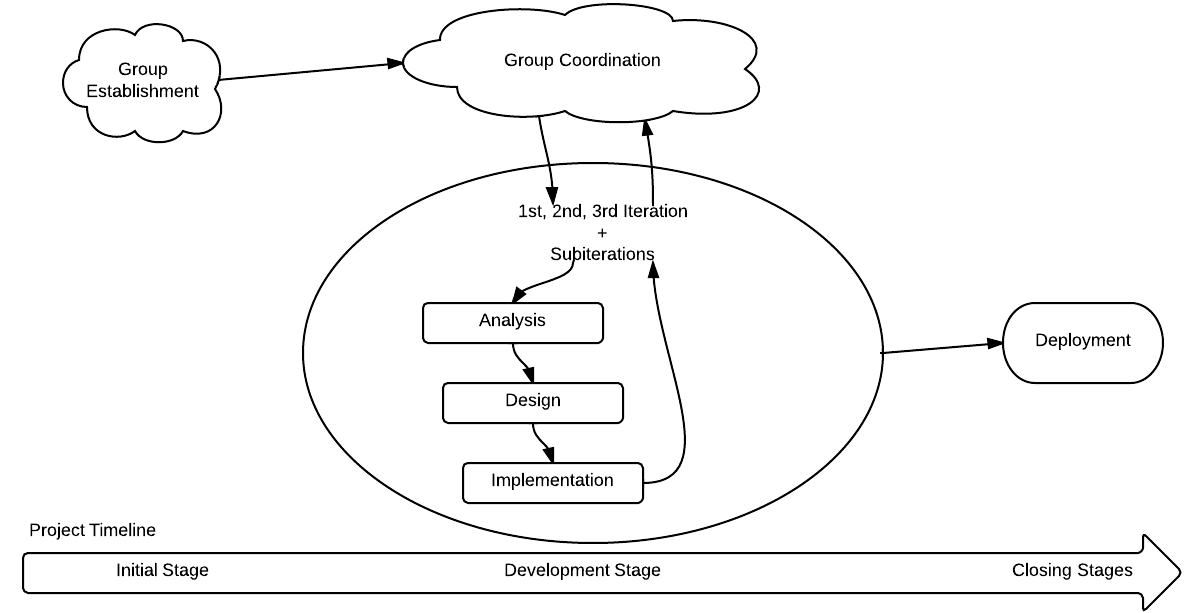
\includegraphics[width=\columnwidth]{images/workflow.png}
\caption{A generalized view of our workflow process}
\label{fig:workflow}
\end{figure}

Each of these illustrated elements were important for the process and contains all valuable information. The figure contains a timeline, which chronologically shows how the project evolved. The project went through three overall stages. These are known as the ``Initial Stage'', ``Development Stage'' and ``Closing Stage''.

\subsection{Stages} \label{subsec:stages}

\subsubsection{Initial Stage}
Before kicking off the project and delve into the actual development, we needed to figure out how to handle the group as \textit{one} collaborating team. This part was of high importance due to the fact that we, as students from two different continents, did not know each other at all. The task was complicated by this. One could presume that in a normal work setting at least the different roles in the team would already have been settled. Some are hired to do the backend (developer) and others others to manage the project (project manager). We needed a specific initial stage to cover this part of getting to know each other, figure out roles and knowledge areas. This was internally known as the ``Initial Stage''. The stage created the necessary basis to work from and we could start to move the project in the right direction.

\subsubsection{Development Stage}
During the development stage several iterations of analysis, design and implementation were executed. As the figure shows, the repetitive phases in the development stage is an iterative process. Even though we were through this loop multiple times, we will only describe the three major iterations, in the section below (See sec. \ref{subsec:iterations}). These iterations are coherent with the project plan and present our general approach to the project. All of the three iterations contains multiple inclusive \textemdash by assessing the artefact\textemdash simpler iterations. Describing each iteration in detail would be a some what cumbersome process.

The reasoning for choosing three major iterations was to accommodate the overall deadlines for the project. Each deadline requested different material containing information about different levels of the project. The first deadline was focused on the requirements and motivation. The second delivery focused on related work and model. Third delivery's focus was on the actual product and its code. These deadlines were a part of our overall project plan and thus led to having three overall deadlines. Initially our goal was to have four major iterations but this was changed due to our unsuccessful efforts to include our colleagues from Kenya. The postponement of deadlines and a general patient attitude caused us to eliminate one major iteration. 

The development stage contains furthermore a group coordination phase. The coordination is reached multiple times throughout the iterations. During this phase important topics were covered, such as sharing status, separation and distribution of tasks, figure out how to proceed, discuss upcoming challenges and the likes. Multiple collaboration methods and tools were used throughout this coordination phase (See \ref{sec:collaboration} and \ref{sec:tools}).

\subsubsection{Deployment Stage}
The deployment stage was considered the simplest and easiest to handle stage of our process. Upon reaching agreement that the development was finalized, the product was deployed to our server. This concluded our work on the product and finalized the development.

\subsection{Iterations} \label{subsec:iterations}
\subsubsection{First Iteration}
Our focus during the first iteration was to get the group work to flow and figure out how to handle the data services provided by the Danish university. Most of the iteration was related to get to know each other and figure out how to move the project forward. The artefacts produced here was of lower level, such as diagrams of the group members programming skills, use case diagrams, first thoughts of domain model, early prototypes of the frontend interface and early implementations of the data services.

It was difficult to really push the project forward at this phase. We used different means of communication with the Kenyans, but without any positive result. Our best result was reached when two out of four African members replied to our emails. No feedback, replies, comments or the likes was received from the two last members.

\subsubsection{Second Iteration}
During the second major phase the groups communication platform and general condition was stable - but unfortunately without any involvement from our Kenyan team members. We knew that we had to push the project forward, and had already wasted too much time on the effort to engage and activate unresponsive members. We were behind our project plan in an attempt to give them enough time to respond, without any luck. We tried to activate one semi-active member from Kenya as a team leader, but his response was, that he was not able to contact the other members.

Our focus changed from here. At the following team meeting we agreed upon, that it would be up to us, to get the project going. We chose to do so because of the fact that we did not receive any kind of feedback from Kenya. We would still let them know every step in the project, and we would continue to try to involve them as much as possible, by emailing them and the likes. We developed multiple artefacts at this point. Our goal through the second iteration was to get a working backend up and running. To do this, we had to chose the best fitting development platform and hereby programming language. The group had to agree on a set of requirements for the engine derived from the requirements in the assignment. The data model was completed and implemented, development of an early working prototype of the backend, and generated several jUnit tests to validate its robustness. Furthermore the work on the frontend started to take form. We did our first evaluation of the frontend (see \ref{sec:usability-test}).

\subsubsection{Third Iteration}
The third and final iteration was a hectic period with focus on getting things done and complete tasks. Because of the earlier effort to activate the Kenyan members, and the time consumed here, we were lacking behind. The now only moderate active member from Kenya chose to leave the group due to personal circumstances. The frontend was implemented with support from data provided by the backend. A second usability test was produced. Also this paper was mostly produced here, by combining bits and pieces and adding lots of new material. Finally the end product was deployed to our server.

During all of the iterations, both major and minor, we used a palette of different methods and tools. These are highly linked with the project phases. The most important are introduced and explained by usage, in the parts that follow below.

\section{Collaboration} \label{sec:collaboration}
A set of different methods were used during the initial stage, in the group establishment, and afterwards in the development stage. These were applied in order to promote and streamline collaboration. Several challenges were met and could have been solved by applying the correct mitigation strategy. The collaboration between the Danish and Kenyan team never evolved enough to engage some of the tactics. The following sections will only highlight the actual engaged methods, and will leave also leave out some methods that are only used briefly. This is done to inform which important actions were taken to engage the Kenyan members and not to blur the picture by which methods that could have been used at a later stage, if the collaboration evolved. For a complete reference of all methods that we sought to use and how they could have been used, see Appendix \ref{sec:collaborationappendix}.

\subsection{Create a common platform} \label{sec:commonplatform}
At the time of the project start we were fully aware that we had several discontinuities, as described by Watson-Manheim et al. \cite{watson2007distance}, between the two groups. Too mention a few, the most challenging were, that we did not share the same culture, time zone \textemdash Kenya was ahead of two hours\textemdash, possibly skills, history and the likes. All of which makes it a challenge to collaborate. One way to solve this is to get to know the different team members in the group. The first step we took in order to make the group work as one unit was to try to create a common ground. The term to create common ground ``refers to that knowledge that the participants have in common, and they are aware that they have it in common'' \cite{olson:2000:distance}. The fact that the members in the teams, local as well as global, had not met each other, or collaborated, before, only stressed the importance of this. In a group like this, where members are spread across different continents, the common ground and the social context that ones behave in, is important. No one knew what to expect from each other, and different cultures introduces different challenges. 

Our approach to mitigate this problem was to email each member, by the email supplied by the coordinators, and introduce the members from ITU. The introduction was superficial and not exhaustive, in order not to frighten anybody. Basic information was listed, such as name, gender, age, contact methods and the likes. This would be a 30 seconds email to compose, and we nonetheless never received any replies. To mitigate this challenge of no replies, we tried to create a spreadsheet listing these simple informations, and expanded it with individual skills significant to the project. It took the Kenyan members close to two weeks to complete this form, while others never completed it.

The reasoning for collecting the members individual skills was to figure out which platform to develop on. In the beginning of the project we talked about the many technologies available for web development. There are many approaches to the same solution, with their pros and cons. Focusing on working as a team, with different members that all have considerably different background experiences we decided to individually write down our development qualifications.

The results were collected and top three choices were joined in a table (See Table \ref{tbl:dev_environment}). Every member then voted for the preferred development platform. One (1) being the preferred approach and three (3) the least preferred. The results are shown below:

\begin{table}[ht]
\caption{Members preferred development platform}\label{tbl:dev_environment}
	\begin{tabular}{rccccccccc}
	& \rotatebox{90}{Kasper} & \rotatebox{90}{Thomas} & \rotatebox{90}{Stefan} & \rotatebox{90}{Rasmus} & \rotatebox{90}{Nicolas} & \rotatebox{90}{Steven} & \rotatebox{90}{Cecil} & \rotatebox{90}{Tom} & \rotatebox{90}{Lucy} \\
		PHP & 2      & 1      & 3      & 3      & 1   &1 &1 &- &1    \\
		C\#.Net         & 3      & 3      & 2      & 1      & 3    &3 &1 &- &3  \\
		Java      & 1      & 2      & 1      & 2      & 2     &2 &3 &- &3  \\
	\end{tabular}
\end{table}

Note: Tom in table \ref{tbl:dev_environment} did not share his experience with the rest of team. Therefore the comparison table was never completed.

One of the challenges in this project was technology readiness \cite{olson:2000:distance}. Every team member has a preferred development language, which ultimately led to a long debate on settling with a development language, and what kind of framework the group should use. The problem was that some team members would have some difficulties participating in the development because of the fact that not all had the same preferred language.

Also some members already had some experience in development of web applications, while others had none or very little. Not everyone was familiar with MVC based development, which for those unfamiliar became a challenge. The overall problem was simply having different level of knowledge regarding web development and technologies.

Ultimately, however, the group decided to go with Java as the main programming language, combined with JavaScript for the frontend. This was chosen due to the fact that java was the most popular in the table \ref{tbl:dev_environment}, and we could not see any limitations with this choice. It ultimately seemed to fit our current needs.

Various milestone for the project was planned and the different implementation tasks, was assigned to different team members. Most noticeable the team created subgroups. The subgroups were divided in teams working with frontend tasks and backend tasks. Frequent meetings and online conversations led to positive awareness \cite{leinonen2005conceptualizing} on what everyone was working with.

The fact that some Kenyan members took several days, and weeks, to reply our emails created a tense feeling in the group. The Danish group had high hopes for the collaboration and were left with a perception of sluggishness towards the Kenyan group. This caused that several members lost trust in the African members, as introduced by Jarvenpaa et al. \cite{jarvenpaa1998communication}. This shows how important the first impression is.

To make it easy to communicate between the group, we created an email list, that every member was a part of. This was done to enable members to create a global awareness in the team and inform each other which challenges we currently faced. We informed every member to use this email. Only a few mails from one member in Kenya was received. The replies were often late and inadequate.

\subsection{Tools} \label{sec:tools}
Generally we used four different tools to communicate our teamwork and progress; one synchronous and five asynchronous. We used Skype for every team meeting and for general communication between the members of the group. Skype is synchronous communication as you will normally receive an instant reply while using voice chat. We furthermore used five asynchronous communication methods, that is GitHub, Email, Google Drive, Doodle and Team Work Project Manager. GitHub was used to share the actual projects current status by communicating via tickets what needs to be done. Email was used for communicating general group announcements, that we want to make sure that all of the members from the group receive. Google Drive to share important documents, such as general to do lists and spread sheet with member interests and skills. In order to mitigate the time zone differences between Nairobi and Copenhagen, that could create problems, we used Doodle to try to sketch up a normal group members week (See appendix \ref{sec:appendix-doodle-schedule}). Doodle is a free online scheduling tool, that automatically takes time zones in to account. One gets presented with a scheme of days and given periods on this day, such as Monday 18th of February, 8:00 to 12:00. Then selects the hours and days that fits. This was done to sketch up the available hours and days that matched the group best. Five Danish members and one Kenyan member filled out this form. It nonetheless told us, that we would have problems meetings different days than Tuesdays and thus had to rely on the other mentioned asynchronous tools to communicate. Finally we used Team Work Project Manager to handle deadlines and milestones, and generally to keep each other informed of the progress. It also includes a Gantt chart that every member could access (see appendix \ref{sec:project-plan}).

\subsection{Global Collaboration Gone Wrong} \label{sec:teamworkgonewrong}
Even though we were only in the early stages of the team work it became quite clear to us that the collaboration was not going to be successful. We only managed to get limited contact with two persons from Kenya, and never managed to either skype chat (neither text or voice) or email with the last two members. One thing that could cause their lack of interaction in our e-mail correspondences and skype meetings are the technology readiness. We know that it is a challenge for some of the group members to get internet access. A recent study shows that only 36,3 \% have access to internet in Kenya \cite{capitalfm2012internet}, which compared to Denmark's 86 \% in 2010 \cite{folketingets-eu-oplysning}, indicates that it is not as easy to get internet access in Kenya as we are used to in Denmark. And we know by fact that a few of them do not have a stable internet connection in their home. 

Our approach to solve this issue was to have a meeting each Tuesday at 10:00 GMT +1. This way we knew that they should have access to their University, which on normal circumstances has an internet connection they could use. We know they should have time for this meeting, thus it is planned as a course on their schedule. Secondly it might have been caused by collaboration readiness. Collaboration readiness is a potential show stopper for any team work, if a given member is not ready to collaborate. There could be many reasons for this, one being that the student was unsure if he or she was going to follow the course. We have tried to identify these issues towards our fellow group members and we cannot find anything that should indicate that they would not be willing to collaborate. They should be just as interested in delivering a good product. We never received any other indication or statement telling us otherwise.

\subsection{Mitigation} \label{sec:mitigation}
We feel, as a group, that we were well prepared for this collaboration. We only got to use a small subset of our methods to mitigate problems due to the fact that no real intentional collaboration effort was there. It is quite obvious to us that no different tactic or set of methods could have solved these problems. If the collaboration had moved from the initial stage, and reached an actual level of real collaboration, one could probably argue that our approach was relied on wrong methods or the likes. But it failed at the early stages, before we had any real impact. These challenges and our thoughts on what could have been done differently will be discussed and reflected in Section \ref{subsec:project}

\chapter{Design}\label{chapter:design}
With inspiration from other building management systems (see Section~\ref{chapter:relatedwork}) and looking at the building simulator we had to communicate with, we came up with the concept of policies that consist of two types of statements; \textit{if-statements} and \textit{set statements}. If-statements works as if-statements in many popular GPL's\footnote{General Programming Language (like C++, Java etc.)}, with a conditional expression, a then-clause and an else-clause. Set statements work by setting a value on the building simulator (in effect it acts as an actuator).

During the initial research for scripting languages we looked at several established embeddable scripting languages (see Figure~\ref{tbl:design-scripting-languages}).

\begin{table}[h]
	\center
	\begin{tabular}{rc}
		\textbf{Name}	&	\textbf{Description}\\
		Python	&	Python scripting\\
		JRuby	&	Ruby scripting\\
		Tcl/Java	&	Tcl scripting\\
		Rhino	&	Javascript scripting\\
		BSF		&	Bean Scripting Framework*
	\end{tabular}
	\caption{Established scripting languages found during research}\label{tbl:design-scripting-languages}
\end{table}

* The BSF supports several languages.

In the team we had some initial discussions if we should use tools that could assist us in designing our own DSL\footnote{Domain Specific Language}. Examples of these kind of tools could be technologies like Xtext~\cite{xtext}, Xbase~\cite{xbase} and EMF~\cite{emf}. Xtext is a framework for developing programming languages and domain specific languages. Xbase is a partial programming language built in Xtext and used for integrating into other programming languages and domain specific languages. Xbase would be able to give us an working expression language. EMF is the Eclipse Modeling Framework, a modeling framework and code generation tool. Some of the team members in the danish group had used those technologies during the ITU course Model Driven Development, but no kenyan team members had any experience with these technologies. This would in effect mean that they would need to acquire the skills learned during Model Driven Development, while simultaneous working and contributing to our joint policy engine project. We deemed this unrealistic. Another argument for not using this set of technologies is that Xbase seemed too daunting a project to undertake due to it's current state. At the time of writing, only 25 questions have been tagged with Xbase on~\cite{stackoverflow} - a website used frequently by the danish team members when in need of coding assistance. The lack of Xbase examples and documentation also reveals that it is a very new, and unfinished, product. Since Xbase would be the caretaker of the expression language, we could have opted to forego just that, and still use Xtext and optionally EMF. We considered this but arrived at the conclusion that using Xtext alone would not give us that much, since our language is small. Also the amount of overhead introduced by using Xtext, both in complexity but also in the generated code, would further add to the confusion of our team members with no experience with this technology. 

Based on the these arguments we chose to develop the functionality ourselves. We also considered that task to be more \textit{fun}! We believe that developing our own scripting language was best given the resources we had available and the timespan of the project. Considering the embeddable scripting languages (see Figure~\ref{tbl:design-scripting-languages}) we only needed a small subset of the functionality (mainly the if-then-else construct) and therefore deemed the complexity versus the timewise return of investment unfavorable.

\section{Architecture}
Merriam-Webster defines \textit{policy} as "A definite course or method of action selected from among alternatives and in light of given conditions to guide and determine present and future decisions".

We have defined a policy as a collection of statements operating on sensors and actuators residing in the building simulator. The policy has a start time and a stop time, indicating when it is active. It is also possible to de-activate a policy completely --- without deleting it entirely --- using a boolean flag.

The system that we have designed consists of four overall parts;
\begin{itemize}
	\item The management website (front end)
	\item The policy engine (back end)
	\item The database for storing policies (back end)
	\item The provided building simulator (back end)
\end{itemize}

Figure \ref{fig:design-system-architecture} illustrates the relationship of the system parts. It is evident that communication between both the front end and the simulator primarily is achieved through Json. For a more in-depth explanation, refer to Section~\ref{subsec:policyengine}.

In terms of MVC\footnote{Model, View and Controller} the \textit{model} and the \textit{controller} is the servlet containing data and business logic. The servlet reacts to several urls (see Figure~\ref{fig:design-servlet-architecture}), that functions as an interface for an operation needed in the system. The \textit{View} is the rendered html based on JQuery.

\begin{figure}[t]
\center{
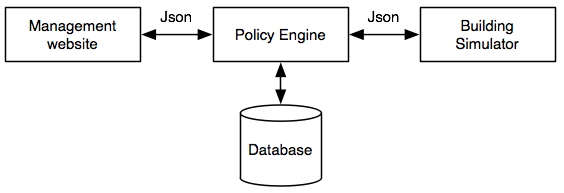
\includegraphics[scale=.5]{chapters/design-system-architecture.png}
\caption{The PolicyEngine system architecture.}\label{fig:design-system-architecture}}
\end{figure}

A statement can either be a SetStatement or an IfStatement. The SetStatement sets an value in the simulator. The backend implementation allows nested If-statements. If-then-else statements have been around possible before even the early versions of Basic, and is an established way of achieving conditional computer logic. Even though the intended audience of our system is not considered computer experts, the if-then-else concept is easy to understand and catches on fast when interviewing people. An If-statement can contain multiple expressions which are being anded when evaluated. If the user wants to make an If-statement with or'ed expressions, she will have to use a nested if. This raises the complexity and we do not consider this to be an optimal solution. The optimal solution in this case would have been to make a proper expression language that is recursion safe, for example based on~\cite{left-recursion}. This would also solve our lacking or's in the condition of the if-statements. Unfortunately we did not realize this until around two thirds into the development. Since our jQuery~\cite{jquery} parsing on the frontend naturally is strongly bound to domain classes on the backend (due to JSon serialization using Gson~\cite{gson}), any big changes at that point would affect both the backend and the front-end. We estimated then that it would be too time consuming to change the system. We therefore leave it up to future work (\ref{chapter:discussion}).

\subsection{The management website}
The management website is a small collection of html pages that relies heavily on JQuery. The building policy administrator opens the main page in a browser, and gets an overview of all the policies and can perform CRUD\footnote{Create, Retrieve, Update and Delete} operations on them.

During the design phase for the GUI of the management website, we used Photoshop sketches that we mailed and transferred via Skype to each other. One from the kenyan team also assisted in this phase. After discussing how to best present policies to the building policy administrator in the time we had available, we choose to use both indentation and color coding page layout (see Section~\ref{chapter:implementation}) when presenting the policies. By choosing this type of GUI, as opposed to a more tabular view on the if's, we elected a GUI that is flexible enough to extend to a recursive rendering which clearly matters a greatly when then-clauses can contain other if-statements that again contain then-clauses and so forth. For implementation see Section \ref{chapter:implementation}.

\subsection{The policy engine}\label{subsec:policyengine}
The policy engine consists of a servlet and domain classes for the expression language needed to build policies. 

A statement can either be a SetStatement or an IfStatement. The SetStatement sets an value in the simulator. The backend implementation allows nested If-statements, making the policies both flexible and simple. 

An If-statement can contain multiple expressions that all are being anded when evaluated. If the user wants to make an If-statement with or'ed expressions, she will have to use a nested if. The optimal solution to this would have been to make an expression recursion safe model. We did not have enough time for this, but we will elaborate further on this subject in the discussion (see \ref{sec:product}). 

The statements are organized as a list. Each statement will be executed (set) or evaluated (if) in the order that they are persisted. Each if-statement has two lists that contain the statements belonging to the then-clause and the else-clause.

The servlet is the core of our policy engine. It has three main objectives;

\begin{figure}[b]
\center{
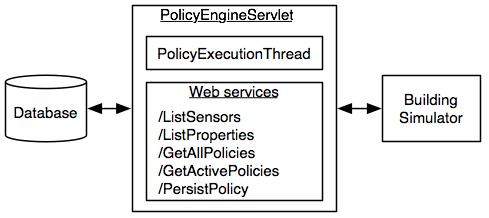
\includegraphics[scale=.5]{chapters/design-servlet-architecture.png}
\caption{A overview model of the PolicyEngineServlet.}\label{fig:design-servlet-architecture}}
\end{figure}

\begin{itemize}
	\item The timed, repetitive execution of policies which currently are active
	\item Serving web service requests to the JQuery front end
	\item Serving the management website html files
\end{itemize}

An overview model of the PolicyEngineServlet can be seen in Figure \ref{fig:design-servlet-architecture}.

The servlet container used is Tomcat 7.0.37\footnote{Other versions might work as well}. 

This design was based on several iterations of group discussions. Everyone wanted a solution that worked efficient and fast, within the loosely defined scope that we initially had set for the system development. And clearly, our project should fit in the timeframe allowed for the project.

The first couple of design proposals from some team members were based on SQL integration --- by the means of creating a java sql connection --- directly into the database that the building simulator uses. This direct integration could be argued as being a good, although strongly coupled integration. Also, it did not feel like a real world scenario (which we are sure that ITU intends as being one of the reasons for this course) if we could access the database directly in this way. Traditionally building systems tend to be closed source proprietary systems with few, if any, integration point. Today there exists different kind of protocols (KNX, LON and BACnet to name a few) that allows some integration to existing building automation systems (for example CTS \footnote{Central Tilstandskontrol- og Styring} systems that are widely used in Denmark). Since our project deals with a building simulator, we do not have to worry about these kind of implementation details --- but we are aware that they exist.

Later design proposals revolved around the idea of having more or less mirrored sensor data in a separate database. Data should be transferred at regular intervals, and the policies should be executed against the copy. This turned out to be a too unsophisticated solution, for several reasons. It would involve a lot of overhead copying data from one database to the other. There is also a problem in knowing exactly what data to copy, since that depends on the statements that is currently active. Based on the above mentioned discoveries we decided on the  following design, that takes all team discussions into account and solves all earlier stated challenges.

On servlet container startup the servlet will read various configuration values, and then set up a thread that manages the timed, repetitive execution of active policies. While testing the system policies were executed every 5 seconds, but this is configurable. The servlet will start by querying the database for active policies, which are defined as policies that have a boolean flag (active) set to true, while the current time is within the policie's \textit{from} and \textit{to} time. This will result in a list of policies that should be executed. Then all sensor id values of all if-statements (including nested statements) are fetched from the building simulator, and cached in an in-memory datastructure. Then the policies are executed, and values set accordingly using the rest API.

\subsection{The database}
The database used is mySQL 5.5.29\footnote{Other versions might work as well} and used for storing the policies. At the moment we only use one table containing all the policies.

\subsection{The building simulator}
The building simulator~\cite{simulator} provided in the course has not been changed or modified in any way.

\chapter{Implementation}\label{chapter:implementation}
%\section{Implementation}
This chapter is dedicated to the implementation of the presented system. In this chapter we will explain in detail what has been implemented and how. 

\section{System}
%%In this section we will elaborate on the implementation for this project. We will delve into the system that the project is running on. We will shortly discuss the technological choices we have made and explain our reasons so.
%%%% Rasmus: Needs to be rewritten. Stupid. What do we want here?
The system has been implemented using Java and Servlets for the backend, and JSP and Javascript for displaying the webpages. We have chosen to use MySQL as a database since it is known to all the members. The database is used to store the policies. 
\\The frontend and backend have been developed to work together as much as possible and the backend to provide all the information necessary for the frontend. However, because we have chosen to serialize the policies to JSON, in the frontend these JSON have to be deserialised and parsed. 
The core part of the system is represented by the servlet that runs the whole application. Inside this servlet there is a timer so policies are executed at a specific interval. The servlet manages all the requests from the frontend and takes appropriate action. 
\subsection{Interfaces}
There are two interfaces that describe the methods of Statements and Value classes. Each statement should implement an execute method, in which specific execution is done. 
\subsection{Domain}
\begin{figure}
	\centering
    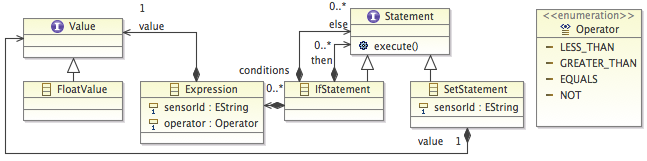
\includegraphics[scale=0.55]{chapters/implementation-model-expression-language.png} 
	\caption{The core classes in the \textit{expression language}.}
	\label{fig:ecore-sensors-actuators}
\end{figure}

A statement can either be a SetStatement or an IfStatement. The SetStatement sets an value in the simulator (in effect it is an actuator). It is possible to have nested IfStatements, making the policies both flexible and simple. An IfStatement can contain multiple expressions that all are being anded when evaluated. If the user wants to make an IfStatement with or between the expressions, will have to use a nested IF. The optimal solution to this would be to make a safe left-recursive model. We did not have enough time for this, but we will elaborate further on this subject in the \nameref{chapter:discussion} section. 

An Expression has three variables, the sensorId, the operator and a value of type Value. When the policy engine is running, each expression is being evaluated. The current value of the sensor is fetched and compared to the desired value using the operator. An expression can contain the following operators; <, >, <=, >=, !=,=. 
If the evaluation of the expression is true, then the statement is executed.

The FloatValue class implements the Value interface and it represents a value of type float. This is used to set the values of the sensors, as those can be of float type. However, because there is no possibility at the moment to set a float value using the REST interface of the simulator, this value is converted into an integer before sending it to the server.

A Policy object consists of statements and the policy can be run by executing those statements. A PolicyEntity object holds a policy and different properties of that policy such as name, description, interval, id and active. The interval property defines from which time to which time should the policy be enforced to run. This is implemented as a separate class, Interval, because of the serialization logics.  The active property represents the status of the policy as in if the user wishes for this policy to be executed (active) or not (not active).
\section{Persistence}
We have decided to have our policies stored in a database. The database chosen was MySQL as it is well known and used by all the members. Because we do not have a complex persistence system, we decided to use the simple JDBC for connecting and querying the database, and not use any frameworks. 
\\Methods for communicating with the database are defined in the DataAccessLayer class. There are the methods for creating, reading, updating and deleting policies. In addition, it is of great interest to have a method that returns only the policies that are running at the current time. 
\\Because the fact that different policies may operate on the same sensors, we decided to use a cache to store each sensor's value. This reduces the number of queries to the simulator server so it does not crash. This cache is implemented using a hashtable and stores the value of the sensor. After executing all the active policies at that moment, this cache is cleared. 
\section{Simulator querying}
To communicate with the simulator's server there is the Connection class for that. It provides methods for connecting to the server and parses the JSON received from it. There are several methods implemented that parse the response of the server and offer information such as - a list with the sensors in a room by providing the room id, a list with all the sensors of a certain type (e.g ac, light, heater etc.) The most two important methods are for retrieving the sensor's value and setting it to a specific one. 
\section{Request Flow}
\section{Front-end}
\label{sec:front-end}

\subsection{Initial Ideas}
We quickly realised that our ideas could easily expand the project, with numerous functionality and features, that would bring the project to a far too complex level.
We mapped all our ideas and prioritized them, and made a selection of ideas, which we planned on implementing.

\begin{figure}[ht]
\centering
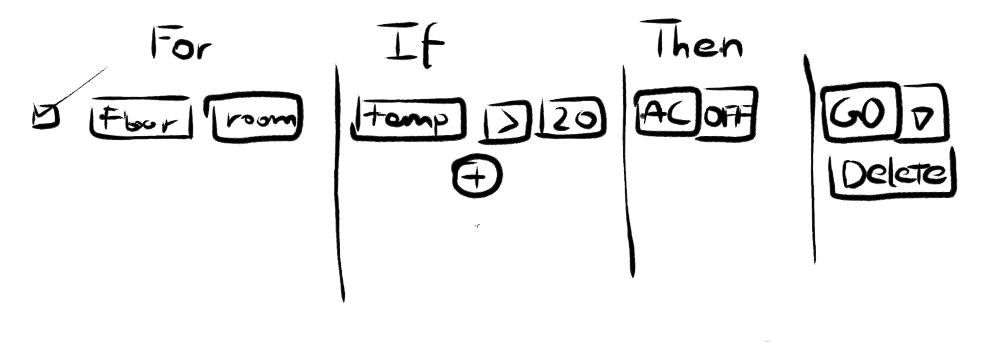
\includegraphics[width=\columnwidth]{initial_idea_frontend.png}
\caption{Initial drawing.}
\label{fig:initialidea}
\end{figure}

The selected ideas that we wanted to realise (sorted by importance) included:
\begin{itemize}
\item Users should be able to add, delete and modify policies.
\item Users should be able to use complex operators in policies, e.g. higher than, lower than, equal to etc.
\item Users should be able to save policies and easily toggle an ON or OFF state.
\item Users should be able to combine multiple sensors in a single policy.
%%%% Aslak: Remember to describe how these wildcards are implemented. In the proper section.
\item Users should be able to use wildcards in a policy, e.g. effecting for instance an entire floor without the need to specify the rooms that belong to the chosen floor.
\item Users should be able to create nested rules in policies.
\end{itemize}

\begin{figure}[ht]
\centering
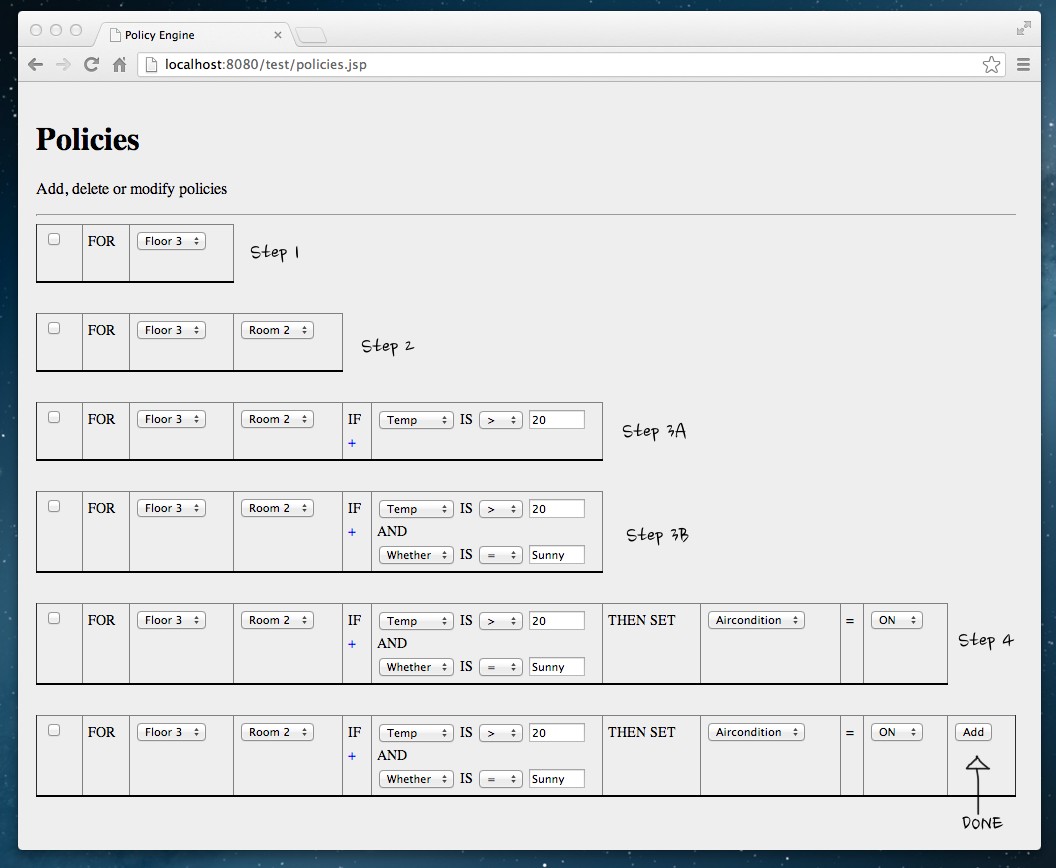
\includegraphics[width=\columnwidth]{building_policy_steps.png}
\caption{Initial drawing - step wise build up.}
\label{fig:initialidea:policysteps}
\end{figure}

All these points where realised in the backend of our implementation, however because of time limits we regret that the possibility to create nested statements did not make it to the user interface. Still we have an interface fully ready to support nested statements, but enabling this feature is something we have added to future work instead. We have started to work on a recursive function to be able to cleverly support endlessly (in theory, computing resources are not endless) deep nested statements. These nested statements would be listed under THEN and would contain a new set of IF, THEN, ELSE subsections. These sections would be easy readable because of indentation and encapsulation.

\subsection{User Interface}
The main goal for the user interface has been to keep it simple and user-friendly without loosing advanced functionality. Initially we made rough drawings to better understand what we were dealing with and how to best possibly present it. Doing so we tried to sketch the process of handling a policy from the creation to the enabling of it. We came up with various approaches, one of them being the step wise (see figures \ref{fig:initialidea}, \ref{fig:initialidea:policysteps}). However this approach proved to be not as flexible as we desired and hard to handle very detailed and complex polices. Our aim has been to make a great overview for the user. Therefore we chose another concept that in which we split each statement up into an open / closeable area to better encapsulate the logic. We believe that it is easier to read one statement at a time, therefore you can keep open the important statements and closed the other ones. Within each statement we also decided to split up IF, THEN and ELSE into subsections because you in theory can add as many entries to each subsection as needed. Nonetheless the introduction of Wildcards allows for manipulation of entire floors, taking up much less space and work for the user to define than having to set up entries for each sensor or actuator on a floor. See an example from the final view of a policy build at figure \ref{fig:statement}.

\subsubsection{Intuitive Design}
What you want to achieve when designing an interface is to make it as intuitive as possible. This can be archieved by looking at the user's "knowledge space" \cite{intuitivedesign}.

\begin{figure}[ht]
\centering
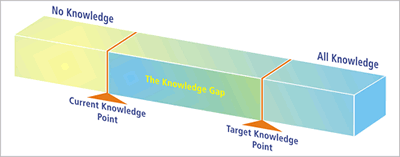
\includegraphics[width=\columnwidth]{knowledge-brick-3.png}
\caption{The space between the Current Knowledge and Target Knowledge points is called The Knowledge Gap.}
\label{fig:intuitivedesign}
\end{figure}

The distance from the left (As seen on figure \ref{fig:intuitivedesign}) indicates how much a given user is familiar with an interface, this is called the "current knowledge point". The next point of interest is called "target knowledge point". This section details how much knowledge the user needs to have to achieve their goals.
Each time a user attempts to perform a specific task, their "current knowledge point" and "target knowledge point" are very important for us to identify.
Each user's "current knowledge point" and "target knowledge point" will be different when they gain more experience. However, it turns out that, by making usability tests we can often identify groups of users who have almost the same "current knowledge point". This is also why we have performed think-aloud tests presented in \ref{sec:usability-test}.

"The Knowledge Gap", which is the distance between the "current knowledge point" and the "target knowledge point", is also called "The Gap".
"The Gap" is what you have full focus on designing for. There is no need to design to the left of the "current knowledge point" and you do not need to design to the right of the "target knowledge point" since the user does not need the knowledge to perform the task. Therefore the focus should be only on designing the interface for the space in between the two points.

Users can accomplish their goals when the "current knowledge point" is equal to the "target knowledge point". There are two ways to achieve this. One way is to train the users, thereby increasing their current knowledge, until they know everything they need to do the job. The other way is to design an interface that can reduce the "current knowledge point" by making the interface more accessible until the "target knowledge point" requires only the information the user already has.

\subsubsection{Flow}
We have strived to create an interface that provides a good flow to the user. The user should not notice the interface but have full focus on the task to be solved - the interface should be transparent. Any distraction breaks the flow. \cite{alancooper}

\begin{quotation}
"No matter how beautiful, no matter how cool your interface, it would be better if there were less of it."
- Alan Cooper
\end{quotation}

There are three prerequisites for achieving flow:

\begin{itemize}

  \item The user must have a clearly defined goal.
  \item There must be a good balance between the user's skills and challenges the user must deal with.
  \item There must be clear and immediate feedback.

\end{itemize}

Especially the last point of the 3 above can be difficult to achieve, when you are in an online environment with response times. However, we believe that we have solved this by allowing the user to model their policy without any server interaction until they want to save.

\subsubsection{Response Times}
In order for the user to get the best possible experience on a website, it is important to optimize response times. Below is the overview of user's reactions at different response times from Alan Cooper - About Face 3:

\begin{quotation}
Up to 0.1 seconds
\\Users perceive the systems response to be instantaneous
\\0.1 – 1.0 seconds
\\Users notice a delay, but their thought processes stay uninterrupted
\\1.0 – 10 seconds
\\Users regard the system as slow, and their mind is likely to wander
\\After 10 seconds
\\The system will loose the users’ attention. They start doing other things or switch to another application
\end{quotation}

Based on this it is important to optimize the web site, both for the code generated on the server, but also to optimize the front-end since around 80\% of the load time \cite{responsetimes} of a website is spent on parsing the generated HTML document, execute javascript and download any external resources. There are a number of things you can do, which we will not go in detail with but just touch on. A few points we are aware of is where and in what order javascript and css is located and loaded, javascript can be loaded last as javascript usually is loaded after a page is fully parsed. Furthermore, you can set preferences for cache and reduce the number of external files to load in an application by combining various javascript files into one and also combine CSS files. 

\subsubsection{Color Coding}
\label{colorcodinglabel}
Color can be a powerful tool to improve the usefulness of an information display in a wide variety of areas if color is used properly. Conversely, the inappropriate use of color can seriously reduce the functionality of a display system \cite{colorcoding}.

We are using color contrasts to express information. We have used this concept to color the different boxes under a statement to improve the readability. 

We have taken into account that red-blue and yellow-blue color combinations are generally safe for color blind people. Having this in mind can lead to a much higher ability to use color coding effectively. This will still cause problems for those with monochromatic color blindness \cite{colorblind}, but it is still something worth considering.

\subsubsection{Responsive Design}
Responsive web design is a web design approach aimed at crafting sites to provide an optimal viewing experience, easy reading and navigation with a minimum of resizing, panning, and scrolling across a wide range of devices (from desktop computer monitors to mobile phones). While we haven't directly optimized for mobile we have had the responsive design idea in mind when setting up the design. What we have assured is that the policy editor is adjusted to the screen size of the user. Meaning if you for instance use a full HD resolution (1920x1080) the interface will utilize this space and boxes with expressions will position themselves accordingly (see example on figure \ref{fig:statement}).

\subsection{Policy Editor}

\subsubsection{Managing Policies}
\label{managing-policies}
In order to make it simple and fast to manage a policy we have split up the interface into sections and sub sections. There are two sections: Policy Information and Policy Statements. In Policy Information, all the content: name, description and time interval are defined. Also the policy can be set to be active or not in this section. The Policy Statements section is where all the expressions are constructed. We have added a sub section for each statement to improve the readability and overview of what is executed and what is paired together (see figure \ref{fig:policy}).  

\begin{figure}[ht]
\centering
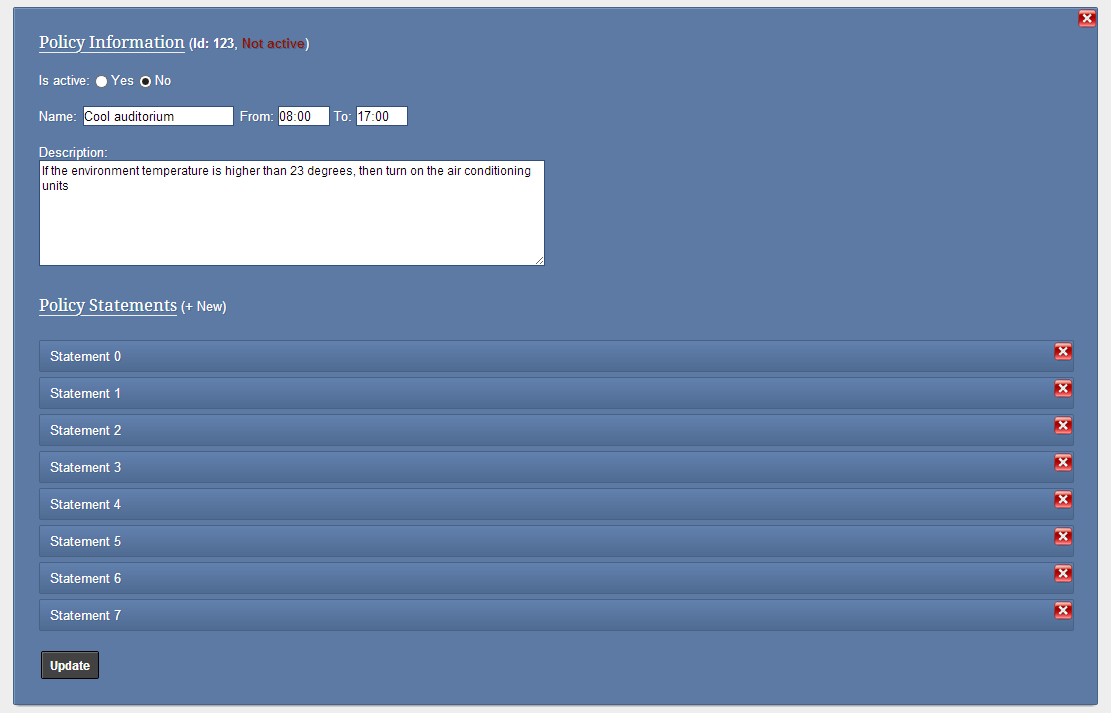
\includegraphics[width=\columnwidth]{policy.png}
\caption{Editing a policy.}
\label{fig:policy}
\end{figure}

Within a statement there are three sub sections: IF, THEN, ELSE (see figure \ref{fig:statement}). For each headline in this setup there is a "+ New" button that can be clicked. This will add a new entry to this particular area. While this is done we alter the policy Javascript object in the background so once the user is satisfied with the setup of statements, it can be saved with a click on the update / save button.

To help the user find the correct sensor / wildcard option, we have implemented an auto-complete functionality. This lets the user start typing a value and then the auto-complete will come up with all the matching elements available.

To make it take less space and work to define a statement that should apply to an entire floor or room, we have introduced wildcard options. All wildcard options are manipulating more then one element all start with "wildcard". A use case for a wildcard can for instance be: A user wants to work with the blinds on the entire first floor: wildcard-floor-1-blind-setpoint is then the option to pick.

\begin{figure}[ht]
\centering
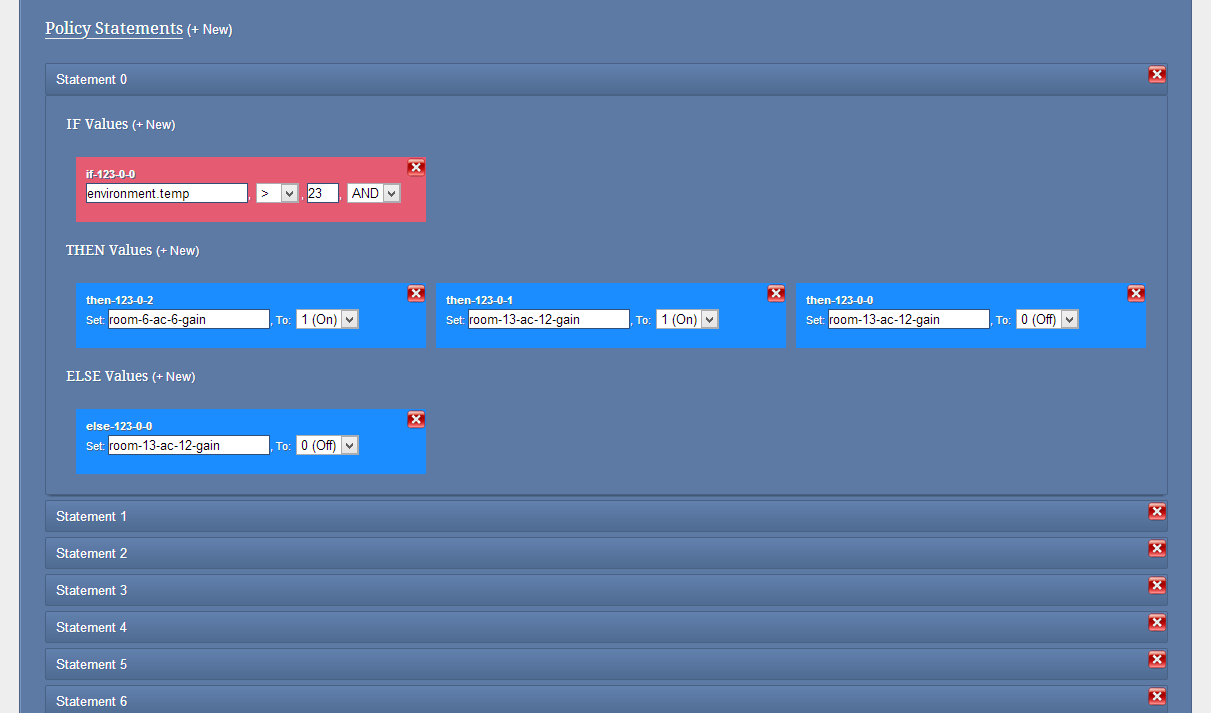
\includegraphics[width=\columnwidth]{statement.png}
\caption{Configuring statements.}
\label{fig:statement}
\end{figure}

\begin{figure}[ht]
\centering
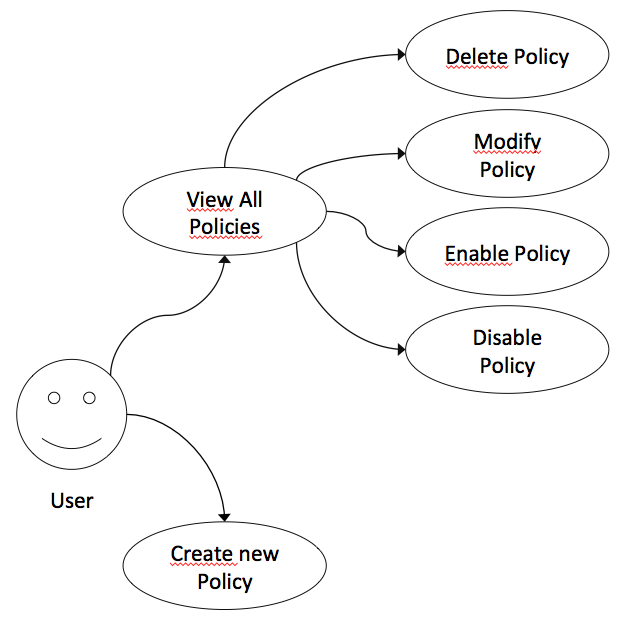
\includegraphics[width=\linewidth]{use-case-diagram.png}
\caption{Use case diagram.}
\label{fig:usecasediagram}
\end{figure}

%%\begin{figure}[ht]
%%\centering
%%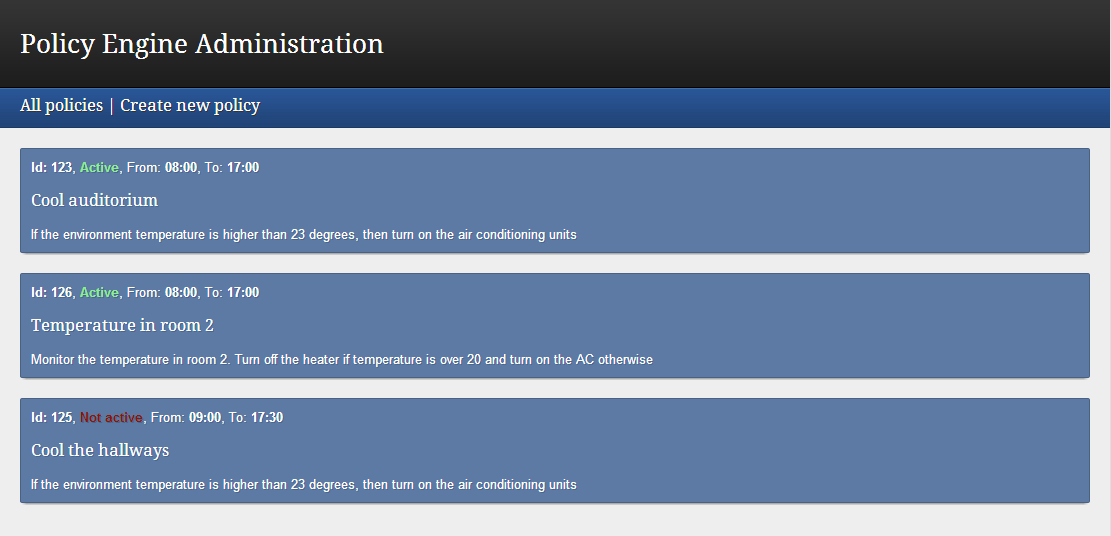
\includegraphics[width=\columnwidth]{policylist.png}
%%\caption{Illustrating the policy list-view.}
%%\label{fig:policylist}
%%\end{figure}

\subsection{Use Case View}
The solution's final use case diagram is shown in Figure \ref{fig:usecasediagram}.

The user starts on the policy list view. Here the user have two possible paths to take: Modify a policy or create a new. Within a policy you can modify details, enable / disable it, setup expressions or delete it.  

\subsection{Usability}
Seeing policies as rules for rooms in a building, with multiple sensors in each and every room, that can affect multiple actuators - not only in one room, but all of the rooms in a building: It leaves the user with a lot of selections. 
This will, if not represented properly, complicate the process of adding new policies.

Following the principles of Steve Krug's "Don't Make Me Think: Common Sense Approach to the Web"\cite{Krug:2005:DMM:1051204}, the functionality of a website should always let users accomplish their intended tasks as easy and directly as possible.
Throughout the development of the front end site we have strived to do so. And we have had two usability tests (more on this in the \nameref{chapter:evaluation} part) to uncover potential problems.

\subsubsection{Browser Compatibility}
We have optimized for modern web browsers. The specific browsers we have tested our solution in are: Internet Explorer 9 and 10, Firefox, Chrome, Safari. 

\subsubsection{Layers of Abstraction}
We have focused on the Visual UI layer enabling a graphical representation of the CRUD (Create, Read, Update Delete) process. Another approach is having policies handled in a textual manner, and thereby forcing users to a write the statements in a policy, using a domain specific language. For a developer textual editing and console commands might be preferred, and may somewhat be quicker, while they know the inputs by heart. But the intended users of our policy engine, are most likely not developers or fans of typing in commands.

In a future version of the policy engine, both methods could be implemented to function in parallel, giving a user both choices, and also the capability of copy and paste policies quickly.

\chapter{Evaluation}\label{chapter:evaluation}
We have evaluated two main areas;
\begin{itemize}
	\item The functional solidity --- using log files and JUnit~\cite{junit} tests
	\item The front-end usability --- using the Think Aloud Protocol
\end{itemize}

Clearly, both areas are important for a successful software system. 

\section{Functional Solidity}\label{policy-engine-system-evaluation}
JUnit tests are structured, assertable software tests that ensures that the software behaves as expected. Of course TDD\footnote{Test Driven Development} --- which we employed using the development of the core functionality --- has it's limits, mainly with regards to the quality of the written tests. The JUnit test accounts for the low level implementation tests.

On a higher abstraction level, we employ log files for testing. A log file is being generated at run-time, and has been integrated into (amongst other areas) the expression language. An example; we already know a certain policy's expected behavior (because we defined it ourselves) --- then we make sure that the policy is executed by the policy engine, and after the successful execution we carefully study the log file and compare it with the expected behavior. We find the log tests a natural selection on top of the more low level automated JUnit tests. It gave us a sense of extra security in regards to the behavior of the policy engine.

\subsection{Log Testing}
\label{log-test}
We have logged system data which was important as to determine if the system was working correctly. Doing so we have been able to verify the behavioral results and to discover bugs in our implementation --- which we then iteratively corrected. 

We have also been using the log files for source code quality control. We verified our solution by cross-referencing every action during tests, and matched it with the actual data stored in the database.

One excerpt from the log file can be seen in figure \ref{fig:log}

\begin{figure}[ht]
\centering
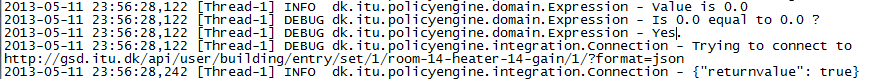
\includegraphics[width=\columnwidth]{images/logoutput.png}
\caption{An excerpt from the log file.}
\label{fig:log}
\end{figure}

\subsection{JUnit Testing}
To strengthen the solidity of the software, and minimize time used on debugging, we implemented a suite of JUnit Tests. An snippet of JUnit code can be seen in \ref{fig:junit-example}. Entering this test, the \textit{ROOM1\_HEATER} has been set to 1 and \textit{ROOM1\_TEMPERATURE} has been set to 26. The purpose is to see if the underlying expression language will set the \textit{ROOM1\_HEATER} to 0, which it should because the Expression's condition is using the \textit{Operator.GREATER\_THAN} along with a value of 25.
 
We have employed a sufficient amount of JUnit tests, to test all operators and both IfStatements (including nested capabilities) and SetStatements.

The result was that our IF-THEN-ELSE concept implementation performed as expected.

\begin{figure}[ht]
\centering
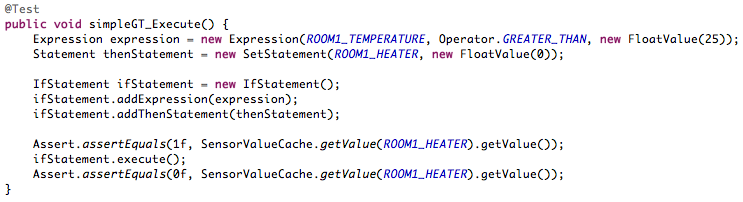
\includegraphics[scale=.5]{images/junit-example.png}
\caption{A snippet of a JUnit test.}
\label{fig:junit-example}
\end{figure}

\section{Usability Test}\label{sec:usability-test}
By using the Think Aloud Protocol we tested to uncover potential usability issues that needed solving.

To evaluate on the usability of our policy engine we decided to make a test with participants outside of our development group. In general, when it comes to "best practices of usability tests", the Think Aloud Protocol is considered one of the most valuable \cite{Nielsen1993}.

The Think Aloud Protocol is time wise inexpensive and easy to set up and it also gives very valuable result from real-life scenarios.

\subsection{Think Aloud Protocol}
In a Think Aloud Test, you ask test participants (one at a time) to use the system while continuously thinking out loud --- that is  simply verbalizing their thoughts as they move through the user interface, and take actions.

To run a basic Think Aloud usability study, three things are required:

\begin{itemize}
\item Recruit representative participants.
\item Inform them of representative tasks to perform.
\item Avoid interference and let the participants speak their actions.
\end{itemize}

We invited five people to each Think Aloud Test. Research shows that having just five people will potentially uncover 80\% of all usability problems \cite{jakobnielsen2000fiveusers} as seen on \ref{fig:usabilitycurve}.

We conducted two Think Aloud Tests, these tests were aimed at fixing any usability issues found during the third iteration.

\begin{figure}[ht]
\centering
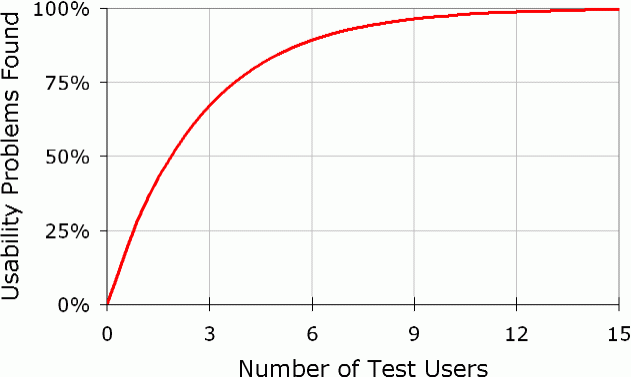
\includegraphics[width=\columnwidth]{usabilitycurve.png}
\caption{Usability test graph.}
\label{fig:usabilitycurve}
\end{figure}

We have not directly targeted Facility Managers in our usability tests, as we simply did not have the time to gather enough test persons with a relevant job function. However instead we gathered a broad range of random test persons with different backgrounds and age.

\subsubsection{Tasks}
We arranged 10 tasks for the participants to perform. Note however that the tests where held individually, but they were all given the same set of tasks. 
During the tests, participants where only given one task at a time to focus on - using small task cards.

Before the test started we explained the purpose of the policy engine, and verbally gave them an example of a user scenario.

We briefly introduced the participant to a map of the building and the rooms involved. We also gave an example list of sensor and actuator names to make them familiar with the elements involved, including basic knowledge of IF, AND, THEN statements and wildcard operators. The questions were designed so that the test persons used all of the features available in the policy engine. The user interface contain an \textit{live auto-complete function} so that the participant can easily set a desired sensor/actuator without knowing the exact name. See section \ref{managing-policies} for more details.

The participants where assigned the following tasks:

\begin{framed}
Create a policy that turns the AC on in Room 1, 1. floor and name it "Cooling".
\end{framed}
The 1st task was designed to see how the participant would try to create new policies - and how they would set the name.

\begin{framed}
Modify the "Cooling" policy just created to affect both Room 1, 1. floor and Room 2, 2. floor.
\end{framed}
The 2nd task was designed to see how the participant handled modifying an existing policy.

\begin{framed}
Create a policy that turns on blinds in all rooms for every floor in the building and name the policy "Sun".
\end{framed}
The 3rd task was designed to see how the participant handled the "wildcard" auto-complete feature.

\begin{framed}
Find and show the active policies just created.
\end{framed}
This 4th task showed how well the participant handled the listing of active policies --- as this would likely be a typical reoccurring task for a building administrator.

\begin{framed}
Disable the policy named "Cooling" so that it is no longer in function.
\end{framed}
The 5th task showed how well the participant handled enabling/disabling of a policy.

\begin{framed}
Delete the policy named "Sun".
\end{framed}
The 6th task showed the removal of policies.

The tasks 7-10 were designed to be harder and the participant was forced to work with complex expressions.

\begin{framed}
To save energy the university wants to have the heating turned OFF automatically at 17:00. However this Wednesday around 19:00 - 22:00 an exclusive presentation is held in room number 5 on 1. floor.
You are asked to maintain a temperature at 21 degrees in that room throughout the presentation.
\end{framed}

\begin{framed}
It is summertime and the overall temperature inside the building is rising. You are asked to keep the temperature at maximum 22 in all of the rooms in the building.
\end{framed}

\begin{framed}
All afternoon between 12:00 and 16:00 the sun is at its peak. Therefore you are asked to set blinds ON in all the rooms on 1. floor and 2. floor - but only if the lights are ON.
\end{framed}

\begin{framed}
The university wants to save energy. You are asked to make sure lights are automatic turned OFF at 17:00 in all the rooms, except from those on 0. Floor.
\end{framed}

\subsubsection{Results and Comments}
\label{results-and-comments}
After every participant had gone through the Think Aloud Test. We went through all their "thoughts" and issues. Some were the same, these we combined into one.
For all the remarks, we made some comments as listed below --- including the actions we took to further improve the software.

\begin{quotation}
If there is a lot of statements - which I would expect there will be? Then I think the statement list would be too long. I think it would make it difficult to keep the overview, if say you have 100 statements.
\end{quotation}

The participant were referring to the “detail view” of a policy, from which every statement were listed underneath each other. 

Due to this remark we have implemented an expand function, which instead of listing all the content at once, it now only shows each statement headline as an open / closable area.
 
\begin{quotation}
I think it is difficult to see which one (rule) belong to what (expression).
\end{quotation}

The participant were referring to the setup within a given policy. When a policy contains an IfStatement, the list of conditional expressions, and the then-clause and else-clause created some confusion. The participant found that it was difficult to separate the different parts.

Due to this we implemented the aforementioned color coding \ref{colorcodinglabel}.

In the second Think Aloud Test with five new persons, the result showed that they found the overview better and easier to understand after implementing this encapsulation and color coding.

After the second round of testing we only had some minor changes to do. But overall the participant where comfortable with the usability and had no further remarks.

We believe that there is always room for improvement, and we elaborate on this in the section \ref{subsec:improvements}.

\chapter{Discussion}\label{chapter:discussion}
%\section{Discussion}
\label{sec:discussion}
In this section we are going to discuss our project in three different parts, one being the collaboration with the team members from Kenya, the other being the product and lastly the overall project. We have chosen to analyse each of these areas with an approach of highlighting what could have been done differently and perhaps in a better and more successful way. We will reflect on our choices made during the project and finally also on our learning outcomes.

\subsection{Collaboration}\label{subsec:collaboration}
The collaboration between the students at ITU, Denmark and Strathmore, Kenya, proved to be a rather challenging task. Only one person from Strathmore showed interest in the project, even though this should have been four persons. We believe that this is not caused by our approach towards the students from Kenya but instead by a lack of interest and willingness to work on the project.
With that being said, there could have been multiple ways we could have achieved a better performing team. Our collaboration strategy is still in the early phases due to the fact that we as a group never got to create any real collaboration platform to work from. 
A natural next approach, that we have tried multiple times to do, would be to gather every team member for an online Skype meeting. This way we would be able to, during a discussion of the current project, to develop multiple different subgroups, see \ref{par:ethnocentrism}, in the team, and not just the two general subgroups as Denmark and Kenya. With these subgroups in place, one would have a much better foundation and a more solid team.

\subsection{Product}\label{subsec:product}
(It is difficult to discuss the product when it is not done)
In the section product, we want to discuss our final product. Questions one could ask:

\begin{itemize}
	\item What could be improved?
	\item Prototype?
	\item Future work?
\end{itemize}


\subsection{Project}\label{subsec:project}
(It is difficult to discuss the overall project when we still have one month left)
A general overview of the project:

\begin{itemize}
	\item What was good?
	\item What was not so good?
	\item How would we approach collaboration in a new project? Do anything different?
\end{itemize}





\chapter{Conclusion}\label{chapter:conclusion}

In this project we present our solution of a web-based platform to manage the scheduling of governing policies for a building. This is done by reading and controlling its sensors and actuators. The project group consists of members from Strathmore University in Nairobi, Kenya and IT University in Copenhagen, Denmark.

The general challenge of the project was to develop a prototype of a policy engine, while collaborating in a distributed team. 

We presented our functional prototype which is able to create, modify and delete policies. The prototype executes the policies against a provided building simulator. We have designed the prototype with usability and flexibility in mind, and it aims to be used by people that are not IT experts, but building administrators. This resulted in having a simple and user friendly web interface that is manageable by the end users. 

Another goal of this project was the collaboration with team members from Kenya. This collaboration has not been a success for several reasons. Mainly that the Kenyans did not respond. Not even to simple emails. Every initial step of collaboration have been ignored by the Kenyan team members. A tendency that sadly kept on throughout the entire project development.

We as the group from ITU, and the teaching staff (Supervisor and Teaching Assistants) - could have done things differently as described in section~\ref{sec:discussioncollaboration}. But ultimately, the lack of commitment from Kenya is the reason that the global collaboration failed.

Despite the fact that, the entire software development, was done by only five people from danmark; And that the project was assigned to nine including the Kenyans  - the prototype of the Policy Engine works as we have expected. 

However there is room for some improvements. One feature that we would liked to have implemented, was temporal constraints in the Statement mechanism. This would provide even more flexibility when defining policies.


%%The improvements should not be introduced here. Are they a part of the future work section?

%%%Not the right place: 
% We thank Matias Bjørling, Javier González and Aslak Johansen for their feedback and offered support on the building simulator. 



\bibliography{gsd}{}%\label{bib:gsd}
\bibliographystyle{plain}
\addcontentsline{toc}{chapter}{References}

%%%%%%%%%%%%%%%%%%%%%%%%%%%%%%%%%%%%%%%%%%%%%%%%%%%%%%%%%%%%%%%%%%%%%%%%%%%%%%%%%%%%%%%%%%%%%%%%%%%%%%%%%%%%%%%%%%%%%%%%
%%%%%%%%%%%%%%%%%%%%%%%%%%%%%%%%%%%%%%%%%%%%%%%%%%%%%%%%%%%%%%%%%%%%%%%%%%%%%%%%%%%%%%%%%%%%%%%%%%%%%%%%%%%%%%%%%%%%%%%%
%%%%%%%%%%%%%%%%%%%%%%%%%%%%%%%%%%%%%%%%%%%%%%%%%%%%%%%%%%%%%%%%%%%%%%%%%%%%%%%%%%%%%%%%%%%%%%%%%%%%%%%%%%%%%%%%%%%%%%%%

\appendix

\chapter{Appendix}
%%Do we really need this?
%%\section{Collaboration} \label{sec:collaborationappendix}
Before any actual work could start, one preliminary goal was to figure out how we could make our group work together as one. Actually this challenge is even more so in this project than in a normal work situation: No organization is in order, no predefined roles, no actual project goals and the likes. This chapter will focus on these challenges and how we tried to handle them. 

%%%%% ASLAK: ``We do not need you to cover the structure here'':
%
%We will highlight different methods to create social interaction and understanding. We will focus on how one can rationalize collaboration. Afterwards we will discuss the different tools we used throughout the project life cycle with collaboration in mind. Finally, we will discuss how one can manage a virtual project.\\
%
%

\subsection{Social Context} \label{subsec:socialcontextappendix}
When we discuss the \textit{Social Context}, we discuss the direct milieu in which the person is and how different factors can influence this person. Communication is also a part of the social context, 
%which is not necessarily only between two persons but can be 
between one to many persons, in different time zones, different cultures etc.\\

\subsubsection{Common ground} \label{subsubsec:commongroundappendix}
Our first step to connect to our student colleagues from Kenya was to introduce ourselves via an e-mail and just shortly highlight some common information about each person from ITU, like stating name, age etc. This method is known as creating ``common ground'', as introduced by Olson and Olson \cite{olson:2000:distance}. The term to create common ground ``refers to that knowledge that the participants have in common, and they are aware that they have it in common'' \cite{olson:2000:distance}. Common ground is not only established through simple general knowledge about each participant. It is also created through a person's behaviour and appearance through meetings and conversations. This is often created between persons with the same temper, sense of humor and the likes. We tried to use this method as a way of getting to know our team members, to create a level of understanding and finally to create a stepping stone from which the project could evolve from. The method of creating common ground is an early way of creating a feeling of a unity, and getting to know each other.
%%%%% ASLAK: How? For deciding wehter to trust what they are saying?

\subsubsection{Trust and First Impression} \label{subsubsec:trustandfirstimpressionsappendix}
This initial contact was quite frustrating because of the fact that it was difficult to get a reply from some of the group members in Kenya. Only two members responded on our first e-mail, after some time, while it was rather hard to get in touch with the others. This leads directly to two different considerations in our group work: ``Trust'' and ``First impressions matters'' as introduced by Jarvenpaa et al. \cite{jarvenpaa1998communication}. Trust in group work is, as the term might indicate, a value of how much the different team members trust in each other. How much does one believe that the other team members will deliver their part of the necessary work? How much does one believe that a mail will be answered? How well does the team work together? The trust between the two subgroups, Denmark and Kenya, was relatively low because of the amount -and lack of- replies and general communication. At the time being we only expect one member from Kenya to be online during our team sessions but at the same time we expect everybody from the ITU group to be online at every session. Trust is an important factor in a group setting; it is a foundation and a crucial part to solve. The group work process is highly related to how well the group function. This is also directly coherent from the first impressions that we received from the group from Kenya, with the lack of communication and willingness to participate in the project. 
%It is not in any way rewarding for the group atmosphere not to join group conversations and not replying emails.

\subsubsection{Collaboration Readiness} \label{subsubsec:collaborationreadinessappendix}
The literature for these challenges seems to agree that these sort of problems generally arise from two different topics. One being ``Collaboration- and Technology Readiness'' and the other ``Continuities/Discontinuities''. The latter part will be discussed in the subsequent section, \nameref{subsec:groupwaretechnologiesappendix} (See section \ref{subsec:groupwaretechnologiesappendix}).

Collaboration readiness is a potential show stopper for the team work, if a given member is not ready to collaborate. This could be caused by having conflicts in interest, e.g. one is about to overtake another persons job or the likes. This could cause that the person, who is about to lose his job, not to be ready to collaborate in a productive manner. We have tried to identify these issues towards our fellow group members and we cannot find anything that should indicate that they would not be willing to collaborate. They should be just as interested in delivering a good product. 

One thing that could cause their lack of interaction in our e-mail correspondences and Skype meetings are the technology readiness. We know that it is a challenge for some of the group members to get internet access. A recent study shows that only 36,3 \% have access to internet in Kenya \cite{capitalfm2012internet}, which compared to Denmark's 86 \% in 2010 \cite{folketingets-eu-oplysning}, indicates that it is not as easy to get internet access in Kenya as we are used to in Denmark. And we know by fact that a few of them do not have a stable internet connection in their home. Our approach to solve this issue was to have a meeting each Tuesday at 10:00. This way we know that they should have access to their University, which most of the time has an internet connection they could use. We know they should have time for this meeting, thus it is planned as a course on their schedule.

\subsubsection{Ethnocentrism} \label{subsubsec:ethnocentrismappendix}
A potential threat to the well-being and harmony of the group is known as Ethnocentrism \cite{durnell2004subgroup}. Ethnocentrism is a state of one subgroup, where the members sees that one group as the centre of everything, and every other group will be valued and ranked from this. A subgroup is a group inside a group, some of the group members are part of - but not the whole group is part of. This way it could create some sense of ``Us versus Them'', which is something you definitely want to avoid. One way to avoid this is to create multiple subgroups inside the group. One subgroup could be those who prefers to work with Java and back-end programming, while others prefer jQuery and front-end development. This could be subgroups across the different countries. If you are part of multiple subgroups the feeling of being part of just one group will dissolve, which should result in a more harmonious group.
This way of creating subgroups would be something that you did early on during the initial communication, and something we tried to solve by writing small parts about each other member from Denmark. Unfortunately, we did not receive any feedback from Kenya. This has probably strengthened the feeling of us vs. them, because we do not know much about them. We definitely have a feeling that our group is the centre right now due to the fact that it is only the Danish group that develops and contributes to the project.

\subsubsection{Coupling of work} \label{subsubsec:couplingofworkappendix}
Coupling of work relates to the state of the current tasks and how loosely or tightly coupled they are. A completely loosely coupled work is one you can perform without the interaction and feedback from other persons. A tightly coupled work task is, on the other hand, one you only can perform with other members of the group participating. Our project has evolved from a very tightly coupled project to a more loosely coupled. This was done on purpose. In the beginning of the project everybody had to be at the meetings because of the fact that we had to define which way to move the project. The development life cycle was quite rigid and strict. After the initial phase, where we decided on the platform, chose an architecture etc., more and more tasks became slightly more loosely coupled one. This means that one could start to work on his part of the project without any direct interaction with other team members. This would also allow such a highly distributed team as ours to collaborate in an efficient way. It would just be too inefficient if everybody had to be together at the same time and place every time anything regarding the project should happen. As of right now we communicate through different Groupware Tools (see \ref{subsec:groupwaretechnologiesappendix}) and only meet through one weekly meeting.

\subsection{Collaborative work} \label{sub:collaborativeworkappendix}
Collaborative work across cultures is a challenge. In our case we had to work together 9 people. 4 being from Kenya, a culture and country that we before entering this project, knew little about. As mentioned earlier the social context and the process of creating ``common ground'' with the collaborators is of high importance. The goal was to create a fundamental shared understanding of the task and build up the motivation and the much needed trust for the collaboration to succeed. Cooperative work is defined by Schmidt as ``People engage in cooperative work when they are mutually dependent in their work and therefore are required to cooperate in order to get the work done'' \cite{schmidt1992taking}.

\subsubsection{Articulation work} \label{subsubsec:articulationworkappendix}
Articulation work is the extra activities required for collaboration \cite{schmidt1992taking}. The extra work is the essence of everything that is needed in order to fulfil the task, e.g. coordination of tasks. Articulation work is about who does what, when and where. There are mechanisms of interaction that supports the process -the life cycle of the project- when articulation work cannot be handled through every day social interaction. These mechanisms are for instance: Organizational structures (formal\/informal), plans, schedules and conceptual schemes. 
%%%%% ASLAK - ``Seems largely redundant'': What all these mechanisms have in common is that they all strive to reduce the effort in labour, resources, time, etc. required to handle articulation work. 
Our strategy for the articulation work was to define processes and choose the groupware technologies that supported our cause best possible.
%%%%% RABER: Needs another iteration. The last sentence needs to be explained. 

\subsubsection{Coordination} \label{subsubsec:coordinationappendix}
The more spread out between people and artefacts a task is the more the reach is increased. Increased ``reach'' of a task changes the coordination. Segregation, which is a method to separate a complex tasks to smaller subtasks, is a suitable strategy when a complex task is at hand. By dividing the complex task into smaller tasks you can often solve them concurrently and thereby complete the larger complex task faster. It also allows for more specialised teams to investigate a task at a more detailed level. Therefore we identified a given number of subtasks, by segregating the larger task. This could be to identify tasks such as ``Create DataAccessLayer'', instead of an overall task like ``Create Backend''. This is one of the ways of how we segregated the tasks within our project. Afterwards each group member were assigned to these tasks, who would work closely together, until the given subtask was completed.

%%Therefore we segregated the tasks within our project into smaller more comprehensible tasks. Group members were assigned to these tasks that would work closer together until the task was completed. 

To handle these tasks we created a project plan with deadlines and milestones. 
%%%%% ASLAK - Idiocracy reference: ``to keep track of everything.''
Moreover we agreed on having a status meeting every week, where we would discuss progress, issues, ideas etc. Arranging a meeting where all are able to attend is not always easy. We did manage to meet on Skype at times which took into consideration both the differences in time zones (temporal discontinuities, see \ref{subsubsec:discontinuitiesappendix}) and the fact that people had entirely different classes and work schedules.

With computer supported cooperative work (CSCW), it is impossible to anticipate every contingency. There will always be exception handling. The core challenges and dimensions of cooperative work includes articulation work, adaptation of technologies and awareness. The lack of trust and awareness when you never meet face to face with your collaborators is problematic and requires methods and training when using communication tools. We primarily used Skype to communicate with and made sure to document changes and commits to the code base very detailed. Individuals working together need to be able to gain some level of shared knowledge about each other's activities.


\subsection{Groupware Technologies} \label{subsec:groupwaretechnologiesappendix}
One way to describe collaborative software, is that it is a software designed to help people achieve a common work task within a group. One of the earliest definitions of collaborative software is found in the research paper ``Rhytms, Boundaries, and Containers'' by Peter and Trudy Johnson-Lenz. They describe the software as: ``intentional group processes plus software to support them.'' \cite{johnson1991post}. The definition was first stated in 1974. Many things have changed, especially in the IT business, but the way a group collaborates and the group dynamics has not. Some general terms are still vital to discuss. We find the most importantly used terms in our project to be critical mass, adaptation and adoption process. These three terms and a general overview of the used tools will be explained in the sections below.

\subsubsection{Tools} \label{subsubsec:toolsappendix}
Generally we used four different tools to communicate our teamwork and progress; one synchronous and three asynchronous. We used Skype for every team meeting and for general communication between the members of the group. Skype is synchronous communication as you will normally get an instant reply while using voice chat. We furthermore used three asynchronous communication methods, that is GitHub, Email and Google Drive. GitHub was used to share the actual projects current status by communicating via tickets what needs to be done. Email was used for communicating general group announcements, that we want to make sure that all of the members from the group receive. Lastly we used Google Drive to share important documents.  

\subsubsection{Critical mass} \label{subsubsec:criticalmassappendix}
%%%%% ASLAK: Critical Mass is a well known concept you can expect people to know about. Nice description though! 
%Critical mass \cite{grudin1994groupware} is a sociodynamic that describes the necessary amount of people needed in order for a product to be a success. An obviously comparison can be made to the ongoing battle between the two social media platforms Facebook and Google+. Facebook has gained a lot of users throughout the last ten years, while Google+ struggles to compete with these numbers. The critical mass is best described by highlighting a real life example, which perfectly describes the term. The current situation of Google+ is that it is far behind Facebook, and we have no real use for it. Google are currently working on gaining a sufficient number of users that will make the product necessary for others to use. This is the goal of achieving the critical mass - to gain enough users for others to see the benefit and the reason for using it.

Critical mass \cite{grudin1994groupware} is a sociodynamic that describes the necessary amount of people needed in order for a product to be a success. We have used this quite directly in our usage of groupware technologies, such as Skype and Google Drive. After selecting which tools to use to communicate between the different members, we have made a great deal out of actually using the tools. This has created the critical mass, for each tool, and every member knows that they can reach each other through these, and thus made it necessary for one to use.

\subsubsection{Adaptation \& Adaption Process} \label{subsubsec:adaptationandadaptationprocessappendix}
Adaption and the adaption process, by Tyre and Orlikowski, \cite{tyre1994windows} are two closely related topics that we briefly touched through our project. These terms relates to how well an organization adapts a new technology and how they do it. Some of the problems with new technologies are that human beings tend to have routines that are not that easy to steer away from. This results in a thought of ``Why should I use this new technology, when it works perfect the way I used to do it''. One of the ways we tried to solve these problems was that we chose our tools as a group, and not by enforcing it. This way the majority chose their favourite tool. The adaption process describes how an organization adapts a new tool: The first couple of weeks are extremely important for a successful adaption. If the adaption does not succeed through these weeks it is very likely that the tool will fade out and never be used again. Our approach to this challenge has been that we pushed it to the people who did not know it, and tried to help them with the setup etc. An example of this could be the installation of Eclipse. One of the members from Kenya had some problems, and we all stayed online throughout the process and helped him install it. This way he could push it to his fellow team members in Kenya.

\subsection{Virtual Project Management} \label{subsec:virtualprojectmanagementappendix}
Virtual Project management is about handling the entire project online, in a virtual and decentralized manner, where the users can access the project from any place and contribute seamlessly in developing the solution. We coordinated activities through GitHub: handling the code base, reporting and updating issues as we moved forward. The mode of interaction has mostly been through chat and voice via Skype, and not through face to face meetings. This presented various discontinuities.

\subsubsection{Discontinuities} \label{subsubsec:discontinuitiesappendix}
Watson-Manheim et al. \cite{watson2007distance} examine virtuality in terms of boundaries and discontinuities. They define discontinuities as ``a break or gap in the work context'', or a ``lack of continuity''. They proposed the concept of discontinuities as a general notion to permit a more comprehensive understanding of the many ways in which virtuality can be perceived.
Distance is the most obvious boundary that is encountered in virtual work but it is clear that there are more boundaries such as time, organization, and nationality, which are not usually present in more conventional work settings to the same extent. It is only when those working in virtual settings perceive a boundary to be a discontinuity that it hinders work processes. 

General properties of discontinuities are that they can emerge and change over time as people adapt in the teams. Discontinuities may only affect parts of the work. The typical discontinuities are temporal (working across time zones), geographic work location, work group membership (e.g. who you work with), organizational affiliation and cultural backgrounds. However discontinuities can also be expertise related (novice versus experts), historical (different version of a product), different professions (e.g. developers and researchers) or different technologies.

%%%% ASLAK: Could you elaborate on this? This is reflection and it is very important for you.
%In our group we experienced how the different cultural backgrounds can become a discontinuity. In Kenya if you show up half and hour or an hour later than the time agreed upon, it is seen as okay. While in the Danish culture it is problematic. Also when asking Kenyans for feedback or criticism they are often fine with how it is, this might be because they don't want to cause problems and don't want to appear impolite. 

%%%% REWRITE:
In our group we experienced how the different cultural backgrounds became a discontinuity. After a couple of scheduled meetings it was clear to us that the respect towards group agreements were not as important in Kenya as in Denmark. This became especially clear in regards to scheduled meetings, where the Danes often would only be a couple of minutes late, if any, which was not the case with the Kenyan members. This could be seen as a general cultural difference, or just the few members different respect of these meetings. 

Another cultural difference we encountered was in regards to their view on us as Europeans. When asking Kenyans for feedback or criticism they are often fine with how it is. This might be because they do not want to cause problems and do not want to appear impolite. This could also be a part of their culture as a way to show respect.

The concept of teams varies across cultures and organizations, and how teams are perceived will differ based on the organizational and national cultural attributes of its members, according to Gibson et al \cite{gibson2001metaphors}. It is also critical to note that individuals from different national cultures vary in terms of their group behaviours and communication styles, as Gudykunst specifies it \cite{gudykunst1997cultural}.

\subsubsection{Continuities} \label{subsubsec:continuitiesappendix}
Continuities are the opposite of discontinuities. Continuities are the stable factors in the collaboration that the participants are aware of and consciously act upon, or they may be implicit and unrecognised \cite{watson2007distance}. Often continuities can be described as strategies or factors to overcome discontinuities. 

\section{Howto Access the Policy Engine} \label{sec:howto-policy-engine}
During this project the individual team members have developed and tested the webapplication locally on their own computer using Tomcat Apache 7.0. However a public accessible solution have also been deployed on an Ubuntu server instance in the cloud\footnote{We are using Amazon EC2 for this purpose}.

To access the solution please go to \url{http://46.137.101.196/gsd-pe} in your favorite web browser.

\section{Howto Access the Source Code} \label{sec:howto-access-code}
For the purpose of easy access and collaboration, the team have created an Github account to hold the source code.

To access the source code please go to \url{https://github.com/tkok/GSD-code} 

\section{Requirements}

\section{Tests}

\section{Project Plan} \label{sec:project-plan}
\begin{figure}[ht]
\centering
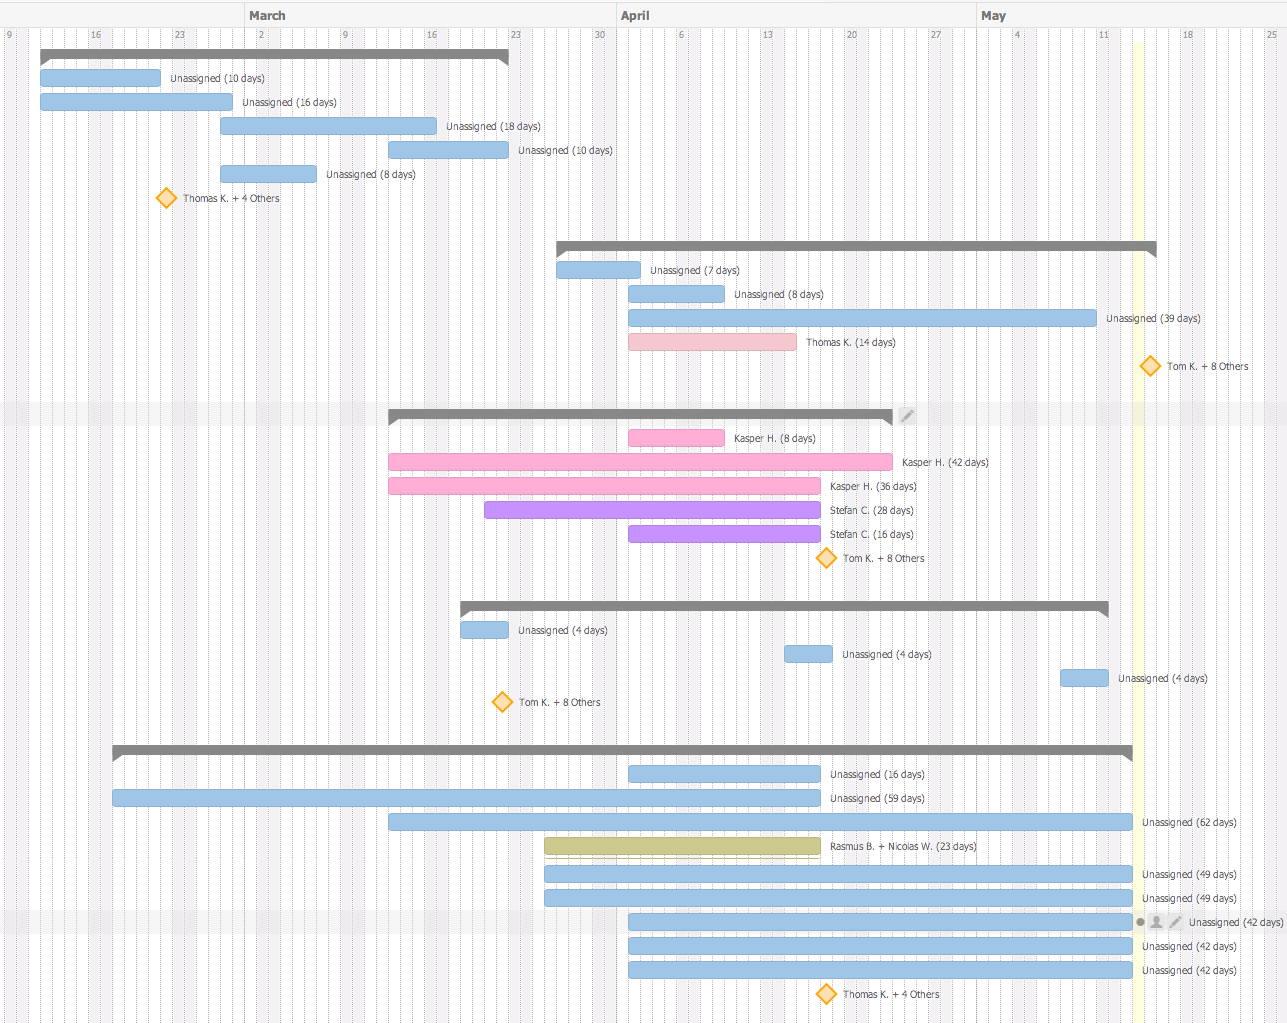
\includegraphics[width=\columnwidth]{images/gantt-chart.png}
\caption{Gantt Chart of the Project Plan}
\label{fig:gantt-chart}
\end{figure} 

\section{Doodle Schedule} \label{sec:appendix-doodle-schedule}
The Doodle schedule shows at which time each participant was able to be online in a collaborative manner. The schedule was only used to create an initial idea of which days each member were available to work on the project. The green boxes shows availability and red boxes unavailability. Each member selected between three time slots for each day in a week. 8AM to 12PM, 12PM to 4PM and 4PM to 8PM. See figure \ref{fig:appendix-doodle-schedule}.
\begin{figure}[ht!]
\centering
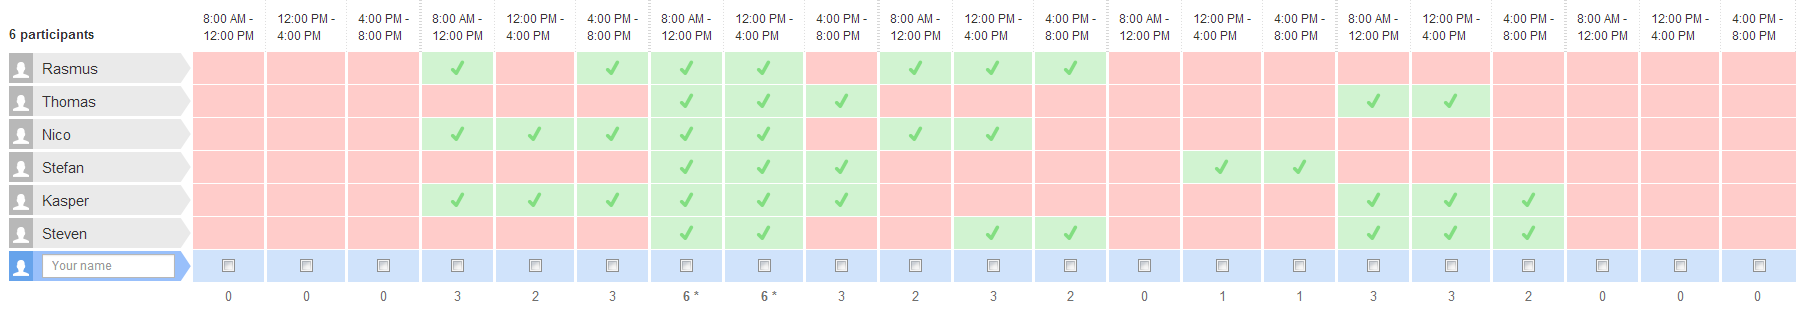
\includegraphics[width=\columnwidth]{images/doodle-plan.png}
\caption{Our Doodle plan showing a normal week from Sunday to Monday. Everybody is available to work each Tuesday.}
\label{fig:appendix-doodle-schedule}
\end{figure}
 


\end{document}

